\documentclass[a4paper]{article}
%\documentclass[aps,prd,preprint,nofootinbib]{revtex4-1}
\pdfoutput=1
\linespread{1}
\usepackage[T1]{fontenc}
\usepackage{amssymb}
\usepackage{url}
\usepackage{graphicx}
\usepackage{xspace}
\usepackage[svgnames]{xcolor}
\usepackage[caption=false]{subfig}
\usepackage{setspace}
\usepackage{amsmath}
\usepackage{listings} 
\usepackage[normalem]{ulem}
\usepackage{placeins}
%\usepackage{braket}
\usepackage{multirow}
\usepackage{tabulary}
\usepackage{hyperref}% add hypertext capabilities
\usepackage{dcolumn}% Align table columns on decimal point
\usepackage{bm}% bold math
\usepackage{soul}
%\usepackage{makecell}

\usepackage[utf8]{inputenc} % utf8 support in source code
\usepackage[a4paper,top=3cm,bottom=2cm,left=3cm,right=3cm,marginparwidth=1.75cm]{geometry}

\usepackage[autostyle]{csquotes} % recommended by biblatex
\usepackage{xpatch} % recommended by biblatex
\usepackage[backend=biber, giveninits, sorting=none, style=numeric-comp]{biblatex} % much more flexible than BibTeX
\addbibresource{bibliography.bib}

\usepackage{siunitx}
\sisetup{separate-uncertainty=true}

\newcommand{\todo}[1]{{\color{red} (To Do: #1)}}
\newcommand{\blue}[1]{\textcolor{NALblue}{#1}}
\newcommand\addcite{[{\color{blue} \underline{CITATION NEEDED}}]}

\newcommand{\enu}{\ensuremath{E_{\nu}}\xspace}
\def\bracketbar{\hbox{\kern-9pt\raise1pt%
    \hbox{{\tiny(}{\lower1.5pt\hbox{\bf--}}{\tiny)}}}}

\begin{document}


\begin{center}
		
	{\Large \bf ProtoDUNE-ND-Tracker: extending the detector physics reach of ProtoDUNE-ND with existing detector components} 
	\vspace*{0.5cm}
	\setcounter{footnote}{0}  
	\def\A{\kern+.6ex\lower.42ex\hbox{$\scriptstyle \iota$}\kern-1.20ex a}
	\def\E{\kern+.5ex\lower.42ex\hbox{$\scriptstyle \iota$}\kern-1.10ex e}
	\small
	\newcommand{\Aname}[2]{#1}
	\def\titlefoot#1{\vspace{-0.3cm}\begin{center}{\bf #1}\end{center}}
	
	\Aname{M.~Auger}{Bern},
	\Aname{R.~Berner}{Bern},
	\Aname{Y.~Chen}{Bern},
	\Aname{A.~Ereditato}{Bern},
	\Aname{D.~Goeldi\footnote{Now at Department of Physics, Carleton University, Ottawa, Ontario, K1S 5B6, Canada}}{Bern},
	\Aname{P.~P.~Koller}{Bern},
	\Aname{I.~Kreslo}{Bern},
	\Aname{D.~Lorca}{Bern},
	\Aname{T.~Mettler}{Bern},
	\Aname{F.~Piastra}{Bern},
	\Aname{J.~R.~Sinclair\footnote{Corresponding author: james.sinclair@lhep.unibe.ch}}{Bern},
	\Aname{M.~Weber}{Bern} and
	\Aname{C.~Wilkinson\footnote{Corresponding author: callum.wilkinson@lhep.unibe.ch}}{Bern}
	\titlefoot{Albert Einstein Center for Fundamental Physics (AEC), Laboratory for High Energy Physics, University of Bern, 3012 Bern, Switzerland\label{Bern}}
	
	\Aname{M.~Bishai}{BNL},
	\Aname{H.~Chen}{BNL},
	\Aname{M.~Diwan}{BNL},
	\Aname{F.~Lanni}{BNL},
	\Aname{Y.~Li}{BNL},
	\Aname{D.~Lissauer}{BNL},
	\Aname{X.~Qian}{BNL},
	\Aname{V.~Radeka}{BNL} and
	\Aname{B.~Yu}{BNL}
	\titlefoot{Brookhaven National Laboratory (BNL), Upton, NY 11973-5000, USA\label{BNL}}
	
	\Aname{M.~Mooney}{Colorado}
	\titlefoot{Colorado State University, Fort Collins, CO 80523, USA\label{colorado}}
	
	\Aname{A.~Bross}{FNAL},
	\Aname{L.~Fields}{FNAL},
	\Aname{D.~A.~Harris}{FNAL},
	\Aname{A.~Marchionni}{FNAL},
	\Aname{T.~Miao}{FNAL},
	\Aname{J.~L.~Raaf}{FNAL} and
	\Aname{J.~Zennamo}{FNAL}
	\titlefoot{Fermi National Accelerator Laboratory (FNAL), Batavia, IL 60510 USA\label{FNAL}}
	
	\Aname{R.~Guenette}{Harvard}, and
	\Aname{J.~Martin-Albo}{Harvard}
	\titlefoot{Harvard University, Cambridge, MA 02138, USA\label{Harvard}}
	
	\Aname{C.~Azevedo}{I3N},
	\Aname{A.~L.~Silva}{I3N} and
	\Aname{J.~Veloso}{I3N}
	\titlefoot{I3N, Physics Department, University of Aveiro, 3810-193 Aveiro, Portugal\label{I3N}}
	
	\Aname{N.~Anfimov}{dubna},
	\Aname{A.~Olshevskiy}{dubna},
	\Aname{A.~Selyunin}{dubna},
	\Aname{S.~Sokolov}{dubna} and
	\Aname{A.~Sotnikov}{dubna}
	\titlefoot{Joint Institute for Nuclear Research~(JINR), Joliot-Curie 6, 141980 Dubna, Moscow region, Russia\label{dubna}}
	
	\Aname{D.~Douglas}{MSU} and
	\Aname{K.~Mahn}{MSU}
	\titlefoot{Michigan State University, Department of Physics and Astronomy, East Lansing,  MI 48824, U.S.A\label{MSU}}
	
	\Aname{M.~Zeyrek}{METU}
	\titlefoot{Middle East Technical University (METU), TR-06800, Ankara, Turkey\label{METU}}
	
	\Aname{M.~Convery}{SLAC},
	\Aname{L.~Domine}{SLAC},
	\Aname{R.~Itay}{SLAC},
	\Aname{K.~Skarpaas}{SLAC},
	\Aname{H.~Tanaka}{SLAC},
	\Aname{K.~Terao}{SLAC},
	\Aname{Y-T.~Tsai}{SLAC} and
	\Aname{T.~Usher}{SLAC}
	\titlefoot{SLAC National Accelerator Laboratory and Stanford University, 2575 Sand Hill Rd, Menlo Park, CA 94025, USA\label{SLAC}}
	
	\Aname{C.~K.~Jung}{Stony},
	\Aname{C.~Vilela}{Stony},
	\Aname{M.~Wilking}{Stony} and
	\Aname{K.~Wood}{Stony}
	\titlefoot{Stony Brook University, Stony Brook, NY 11794, USA\label{Stony}}
	
	\Aname{D.~A.~Dwyer}{LBNL},
	\Aname{D.~Gnani}{LBNL},
	\Aname{C.~Grace}{LBNL},
	\Aname{S.~Kohn}{LBNL},
	\Aname{M.~Kramer}{LBNL},
	\Aname{A.~Krieger}{LBNL},
	\Aname{K.~B.~Luk}{LBNL},
	\Aname{P.~Madigan}{LBNL} and
	\Aname{C.~Marshall}{LBNL}
	\titlefoot{University of California and Lawrence Berkeley National Laboratory, Berkeley, CA 94720, USA\label{LBNL}}
	
	\Aname{B.~Bilki}{Iowa},
	\Aname{K.~Cankocak}{Iowa},
	\Aname{J.~Nachtman}{Iowa},
	\Aname{Y.~Onel}{Iowa} and
	\Aname{A.~Penzo}{Iowa}
	\titlefoot{University of Iowa High Energy Physics Group, Iowa City, IA 52242, USA\label{Iowa}}
	
	\Aname{J.~Chaves}{UPenn} and
	\Aname{C.~M.~Mauger}{UPenn}
	\titlefoot{University of Pennsylvania,Philadelphia, PA 19104, USA\label{UPenn}}
	
	\Aname{S.~Manly}{Rochester},
	\Aname{K.~S.~McFarland}{Rochester} and
	\Aname{D.~Ruterbories}{Rocester}
	\titlefoot{University of Rochester, Rochester, NY 14627 USA\label{Rochester}}
			
	\Aname{D.~Barker}{Sheffield},
	\Aname{A.~C.~Ezeribe}{Sheffield},
	\Aname{T.~Gamble}{Sheffield},
	\Aname{N.~McConkey}{Sheffield},
	\Aname{N.~J.~C.~Spooner}{Sheffield},
	\Aname{M.~Thiesse}{Sheffield}, 
	\Aname{E.~Tyley}{Sheffield} and
	\Aname{M.~H.~Wright}{Sheffield}
	\titlefoot{University of Sheffield, Western Bank, Sheffield S10 2TN, UK\label{sheffield}}

        \newpage
	
	\Aname{C.~Kuruppu}{SC}, 
	\Aname{S.~R.~Mishra}{SC} and
	\Aname{R.~Petti}{SC}
	\titlefoot{University of South Carolina, 712 Main Street, Columbia, SC 29208 USA\label{SC}}

	\Aname{J.~Asaadi}{Arlington} and 
	\Aname{H.~Sullivan}{Arlington}
	\titlefoot{University of Texas at Arlington, Arlington, TX 76019, USA\label{Arlington}}
	
	\Aname{B.~Fleming}{YALE} and
	\Aname{S.~Tufanli}{YALE}
	\titlefoot{Yale University, Wright Laboratory, New Haven, CT 06520 USA\label{YALE}}
	
\end{center}
\vspace*{1cm}

\begin{abstract}

In this document we propose introducing a tracking scintillator detector, ProtoDUNE-ND-Tracker, to extend the utility of the ProtoDUNE-ND proposal over the ArgonCube 2x2-only case, while no other DUNE ND subdetector prototypes are available. ProtoDUNE-ND-Tracker repurposes components of the existing MINERvA and MINOS-ND hardware already positioned on-axis in the NuMI beam, in the same detector hall as ProtoDUNE-ND is to be sited.

Using ProtoDUNE-ND-Tracker paired with the ArgonCube 2x2 Demonstrator, the response of the 2x2 can be characterized as a function of momentum, providing a validation of the momentum measurement via multiple coulomb scattering that will need to be used for side-exiting muons in both the DUNE ND and far detector. Pairing the 2x2 with MINERvA enables a test of the ability to track muons and fast neutrons from the slow and busy LAr detector into a fast-response detector, the keystone of the DUNE ND.

As ProtoDUNE-ND is designed to be easily reconfigurable, with a moveable cryogenic system for the ArgonCube 2x2 Demonstrator an important test of the DUNE-PRISM technical design, the ProtoDUNE-ND-Tracker would in no way preclude the introduction of future DUNE ND subdector prototypes, and is likely to prove invaluable for future reconfigurations of the design.
  

\end{abstract}



% For now suppress the table of contents
%\tableofcontents

\section{Introduction}
\label{sec:introduction}

DUNE is a next-generation accelerator neutrino oscillation experiment~\cite{DUNE, DUNE2}. DUNE will utilize an intense beam of predominantly muon (anti)neutrinos produced at Fermilab, will sample the unoscillated beam on the Fermilab site, \SI{574}{\metre} from the proton target and \SI{62}{\metre} underground, and then will sample the oscillated beam \SI{1300}{\kilo\metre} away and \SI{1.5}{\kilo\metre} underground, at the Sanford Underground Research Facility (SURF) in South Dakota, using four \SI{10}{\kilo\tonne} liquid argon (LAr) target modules. By using LAr time projection chambers (TPCs), DUNE benefits from the exquisite precision to look at the particles escaping the nucleus, and measuring the neutrino energies with unparalleled accuracy. An extensive research and development (R\&D) program is currently ongoing to deliver detectors capable of fulfilling DUNE's physics goals. The unprecedented size of the DUNE far detectors~\cite{DUNE_IDR_v1, DUNE_IDR_v2, DUNE_IDR_v3} has motivated large-scale LAr TPC tests, in the single- and dual-phase ProtoDUNE modules in CERN~\cite{Abi:2017aow, Agostino:2014qoa}, in themselves, the largest LAr TPCs built to date.

As the DUNE far detectors have LAr targets, there will also be a major LAr component for the DUNE near detector suite, in order to minimize cross section and detector systematic uncertainties for oscillation analyses~\cite{DUNE, DUNE2}. However, the intense neutrino flux and high event rate at the near detector makes traditional, monolithic, projective wire readout TPCs unsuitable, which has motivated a program of R\&D into a new LAr TPC approach, suitable for such a high rate environment, known as ArgonCube~\cite{argoncube_loi}. ArgonCube utilizes detector modularization to improve drift field stability, reducing high voltage (HV) and the LAr purity requirements; it uses a pixelized charge readout~\cite{pixels, larpix}, which provides unambiguous 3D imaging of particle interactions drastically simplifying the reconstruction; and new dielectric light detection techniques with ArCLight~\cite{arclight}, which can be placed inside the field cage to increase light yield, and localization of light signals. Additionally, ArgonCube uses a resistive field shell, instead of traditional field shaping rings, to minimize the dead material and maximize active volume, and to minimize the power release in the event of a breakdown~\cite{argoncube_fd}. Such an optically segmented, pixel readout LAr TPC has been recommended as the major LAr component for the DUNE near detector by the DUNE Near Detector Concept Study Group~\cite{dune_ndcsg}.

Early investigations in Bern into long drift lengths and high electric fields with the ArgonTube detector~\cite{argontube_design} found a number of technical issues and a higher than expected risk of breakdowns~\cite{argontube}, as well as testing cryogenic charge readout electronics~\cite{art_cold_ero}. Smaller, modular, LAr TPCs were introduced as a robust solution to the high voltage problem, which reduces the LAr purity requirements due to the short drift lengths, and which have obvious advantages in high multiplicity environments. The feasibility of pixelated readout was demonstrated using a 60-cm-drift pixel TPC located at the University of Bern in 2016~\cite{pixels}. LArIAT~\cite{lariat} has since operated a scaled-up version of this readout technique (renamed PixLAr) at Fermilab in 2017. The recent development of the LArPix pixel readout electronics by LBNL have removed the ambiguities present for the earlier tests~\cite{larpix}. The 60-cm-drift pixel TPC, and a 10-cm version at LBNL, were used to demonstrate cold amplification and cold digitization with the first version of the LArPix electronics~\cite{larpix}. A field-shell demonstrator TPC was tested successfully in Bern in 2018~\cite{argoncube_fd}. Tests of the ArCLight dielectric photon detector have also been carried out in LAr, as described in Ref.~\cite{arclight}. With the various technological developments demonstrated with small-scale TPCs, the next necessary step in the ArgonCube program is to demonstrate the scalability of the pixelized charge readout and light detection systems, and to show that information from separate modules can be combined to produce high quality event reconstruction for particle interactions. To that end, a mid-scale (\SI[product-units=repeat]{1.4x1.4x1.2}{\metre}) modular TPC, dubbed the ArgonCube 2x2 Demonstrator, with 4 independent LAr TPC modules arranged in a 2x2 grid has been designed, and is currently under construction in Bern. Given the environment that the DUNE near detector will operate in, it is desirable to operate the ArgonCube 2x2 Demonstrator in an intense, few-GeV, neutrino beam.


In this document, we propose moving the ArgonCube 2x2 Demonstrator into the NuMI on-axis neutrino beamline at FNAL, to serve as the core of a prototype for the near detector, or ProtoDUNE-ND. This is in analogy to the successful ProtoDUNE program for the far detector. A detailed description of the proposed location and the ArgonCube 2x2 Demonstrator module can be found in Section~\ref{sec:protodune-nd}. A description of the detector physics studies to be performed with the 2x2 alone is given in Section~\ref{sec:detector-physics-studies}. Additional detector physics possibilities if a downstream tracker is added to ProtoDUNE-ND are described in Section~\ref{sec:MINERvA_MINOS}, with the option of repurposing existing MINERVA and/or MINOS ND hardware is discussed. The outlook for the test modules and a timeline in Section~\ref{sec:outlook}. Conclusions are presented in Section~\ref{sec:conclusions}.


\section{Incorporating other detector prototypes into ProtoDUNE-ND}
\label{sec:MINERvA_MINOS}

\begin{figure}[htb]
	\centering
	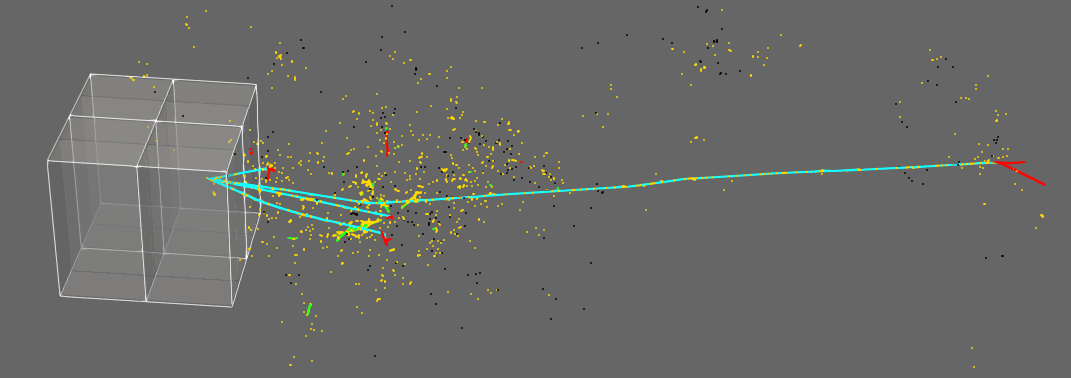
\includegraphics[width=0.8\textwidth]{{plots/EventDisplays/8.17GeV_rectangle_crop}.png}
	\caption{Example ArgonBox simulated event for an 8.17 GeV $\nu_{\mu}$--argon neutral-current multi-pion interaction, in which the pions are not contained in the module. Energy deposits in a bulk volume of LAr are color-coded according to the particle type: $\pi^{\pm}$ --- blue; $\mu^{\pm}$ --- purple; $e^{+}$ --- green; $e^{-}$ --- yellow; proton --- red; recoiling nuclei --- black. The event vertex was randomly placed inside the active volume of the ArgonCube 2x2 Demonstrator, the geometry for which is superimposed on these images, but which is not simulated by ArgonBox.}
	\label{fig:leaky_event}
\end{figure}
Given the ArgonCube 2x2 Demonstrator's size and the relatively high energy NuMI ME beam, many events will not be contained in the 2x2 alone. Figure~\ref{fig:leaky_event} shows a neutral current event where many pions are produced, but in which the pions and subsequent hadronic showers extend far beyond the detector. Indeed, many such events would not be contained in the full ArgoNCube deployment at the DUNE ND, in the LBNF beamline, and for charged-current events, the muon will be uncontained most of the time. For this reason, and because it is not possible to magnetize the large LAr component, further, magnetized, tracking detectors are proposed downstream of ArgonCube in the full DUNE ND complex, and the requirement to tag side-escaping particles is discussed in Ref.~\cite{dune_ndcsg}. Broadly speaking, three additional subdetector options are considered for the DUNE-ND design, in addition to ArgonCube~\cite{dune_ndcsg}, as introduced in Section~\ref{sec:tracking_detectors}: a scintillator tracking detector; a magnetized low-density tracking detector; and a Cosmic Ray Tagging (CRT) system.

Prototypes for these detectors are also being planned, and the ProtoDUNE-ND complex is intended to evolve over time to accommodate them. As has been remarked, the cryogenic system for the ArgonCube 2x2 will be moveable to test key components of the DUNE-PRISM technical design, which will allow ProtoDUNE-ND to be easily reconfigured to accommodate any future prototype detectors. In this section, we discuss how adding those additional detectors will enhance the neutrino engineering studies possible with the ArgonCube 2x2 Demonstrator alone. With multiple subdetectors included in ProtoDUNE-ND, multi-detector reconstruction capabilities can be developed and tested. Additionally, if the sign and momentum of escaping hadrons and muons can be measured, it may be possible to make physics measurements with ProtoDUNE-ND, which would be beneficial to the overall DUNE program.

\subsection{Scintillator tracking detector}
\label{sec:minerva}
Two distinct scintillator options are currently being considered for the DUNE ND design, as introduced in Section~\ref{sec:tracking_detectors}. A large, fully active, Three-Dimensional Scintillator Tracker (3DST), and scintillator components downstream of the HPgTPC to tag escaping neutral particles. %As discussed in Section~\ref{sec:detector-physics-studies}, a large fraction of particles will not be contained in the 2x2 alone. A downstream scintillator detector would recover many of these particles, and would make it possible to benchmark the 2x2 response to a wider range of particle energies, and therefore the expected DUNE phase-space.

To investigate the effect that adding a scintillator component, and generically a downstream tracking detector, to ProtoDUNE-ND, a simulation was performed where a generic scintillator box was included downstream of the ArgonCube 2x2 Demonstrator. Neutrino interactions are generated in the ArgonCube active volume, and propagated through an approximation of the ArgonCube 2x2 demonstrator and scintillator block.  The scintillator detector used is simply a rectangular box, \SI[product-units=repeat]{1.4x1.4}{\metre\squared} in the dimensions transverse to the beam, making it large enough to cover the downstream face of the 2x2 active volume. In the beam direction, the scintillator is split into 

, and~\todo{how long?}  The simulation includes the most downstream 12 modules (24 planes) of the tracker region, as well as the full downstream ECAL and HCAL regions.  The rectangular box represents the central part of the MINERvA inner detector, and is large enough to cover the entire ArgonCube active volume. An example event is shown in Figure~\ref{fig:2x2+MINERvA_event}, and can be compared with 2x2 only events in Figures~\ref{fig:argonbox_event_display} and~\ref{fig:leaky_event}. Note that this simulation only included the ArgonCube cryostat and MINERvA detector components, no material was included outside these (so escaping particles simply leave without ever re-interacting). This is unlike the previously described ArgonBox simulation, where a large box of argon was simulated (so escaping particles still re-interact). Events were again distributed uniformly throughout the ArgonCube active volume.
\begin{figure}[htb]
  \centering
  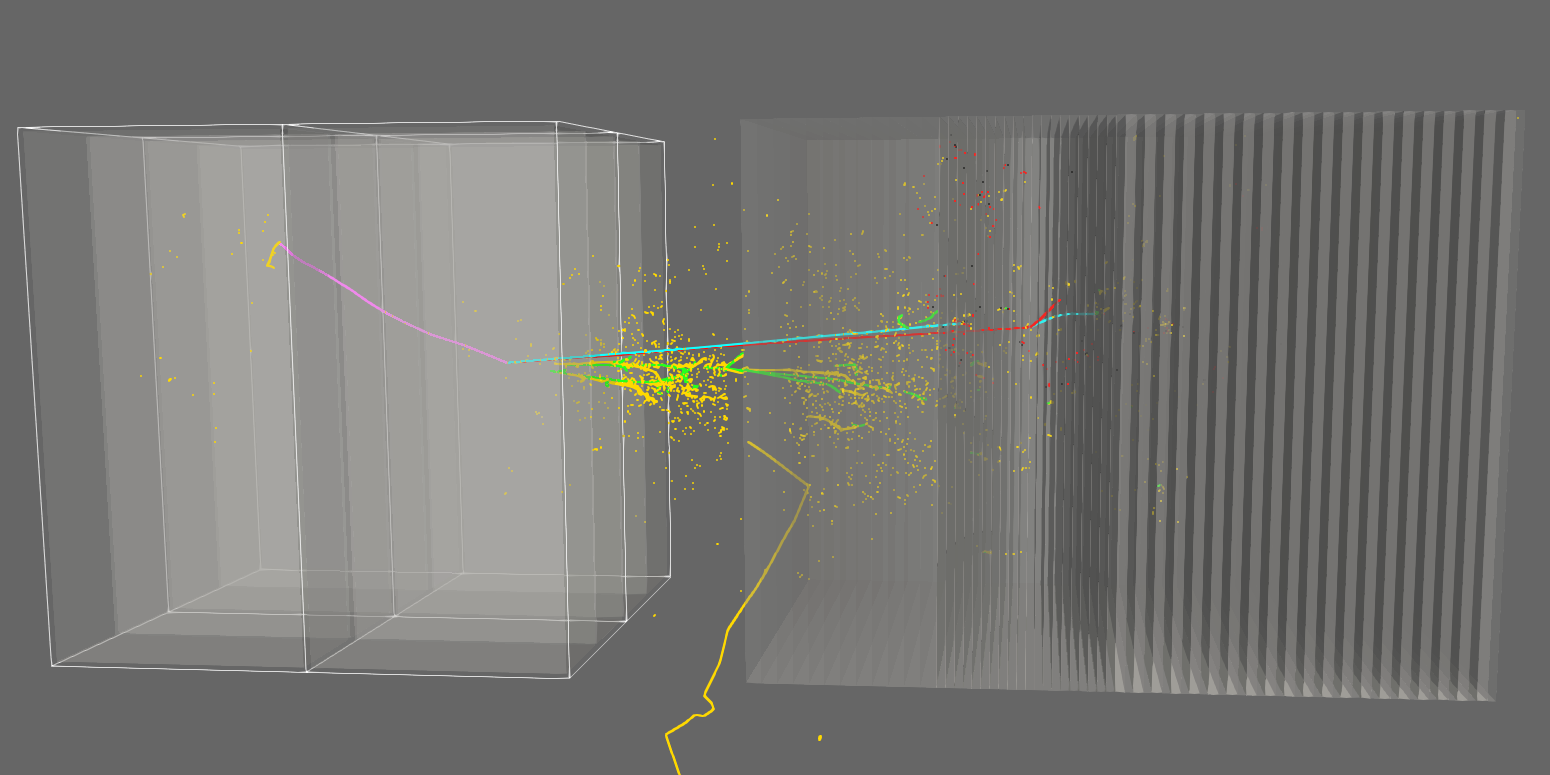
\includegraphics[width=0.8\textwidth]{{plots/Event_Displays_2x2_MINERvA/MINERvA_full_e70_rectangle_crop}.png}
  \caption{Example simulated event for a 7.0 GeV $\nu_{\mu}$--argon charged-current interaction, in which particles not contained in the ArgonCube 2x2 enter the scintillator block detector. Energy deposits are color-coded according to the particle type: $\pi^{\pm}$ --- blue; $\mu^{\pm}$ --- purple; $e^{+}$ --- green; $e^{-}$ --- yellow; proton --- red; recoiling nuclei --- black. The event vertex was randomly placed inside the active volume of the 2x2 Demonstrator module.}
  \label{fig:2x2+MINERvA_event}
\end{figure}

In the following, we discuss potential detector physics studies, or improvements to detector physics studies previously discussed in the ArgonCube 2x2-only case (in Section~\ref{sec:detector-physics-studies}), incorporating elements of the MINERvA detector downstream of the ArgonCube 2x2 module.

\subsubsection{Track matching}
All DUNE ND designs considered in Ref.~\cite{dune_ndcsg} include some fast scintillator component, downstream of the LAr ArgonCube component, and downstream of a low-density GAr TPC tracker, to tag escaping particles, photons, and possibly neutrons. There is a significant reconstruction challenge in matching the escaping tracks from the LAr component, with the signals in the scintillator, given the slow charge readout in the LAr TPC, and the high multiplicity DUNE-ND environment.

\begin{figure}[htb]
  \centering
  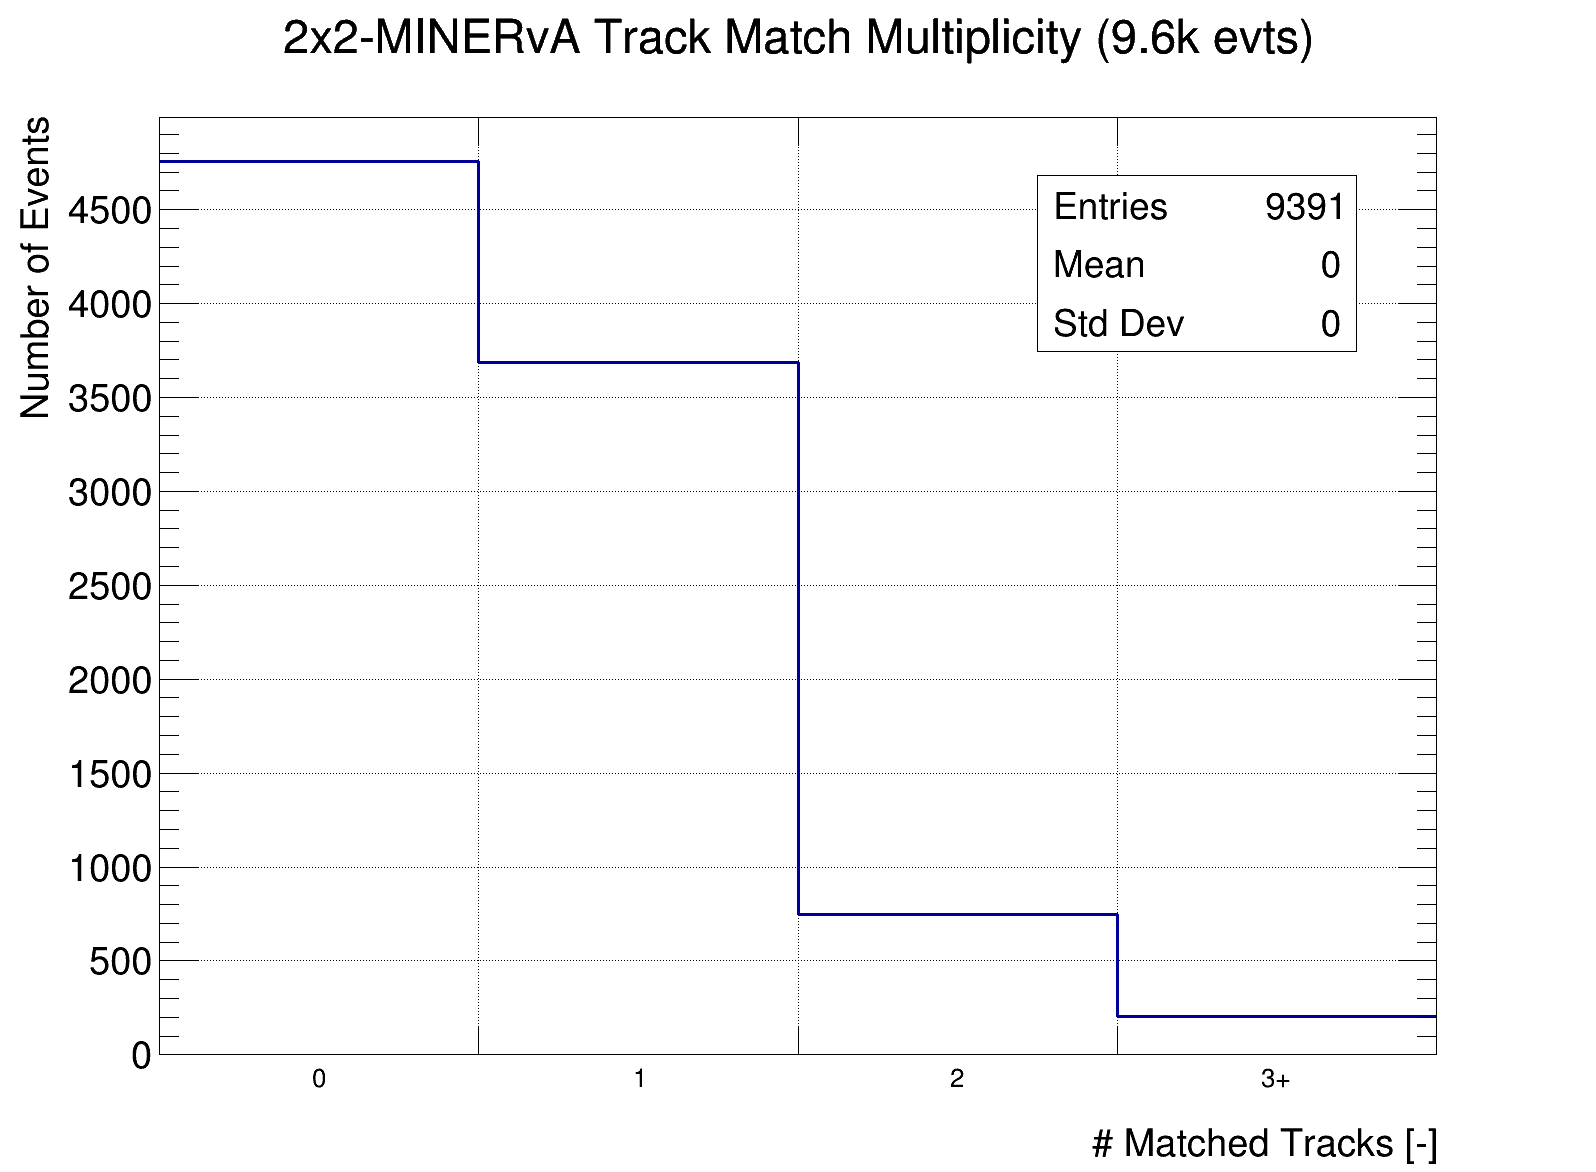
\includegraphics[width=0.6\textwidth]{plots/2x2_minerva_plots/track_mathch_multiplicity.png}
  \caption{Simulated number of true tracks produced by simulated GENIE interactions in the ArgonCube 2x2 active volume, which deposit energy in both the 2x2 module, and the MINERvA component positioned downstream of the 2x2.}
  \label{fig:track_multiplicity_min}
\end{figure}
Many tracks produced in the LAr volume are not contained by the ArgonCube 2x2 module, and the majority will escape downstream. In Figure~\ref{fig:hadronic_containment}, the multiplicity of tracks which deposit charge in both the ArgonCube 2x2 module and the MINERvA component, included in the simulation described above, are shown. Full DUNE-ND events are likely to have an even higher LAr to scintillator track multiplicity due to the pile-up in the much larger 35 t ArgonCube LAr detector. But it is clear from Figure~\ref{fig:track_multiplicity_min} that including MINERvA elements in the ProtoDUNE-ND tests would provide useful data with which to start tackling this reconstruction problem.

\begin{figure}[htb]
  \centering
  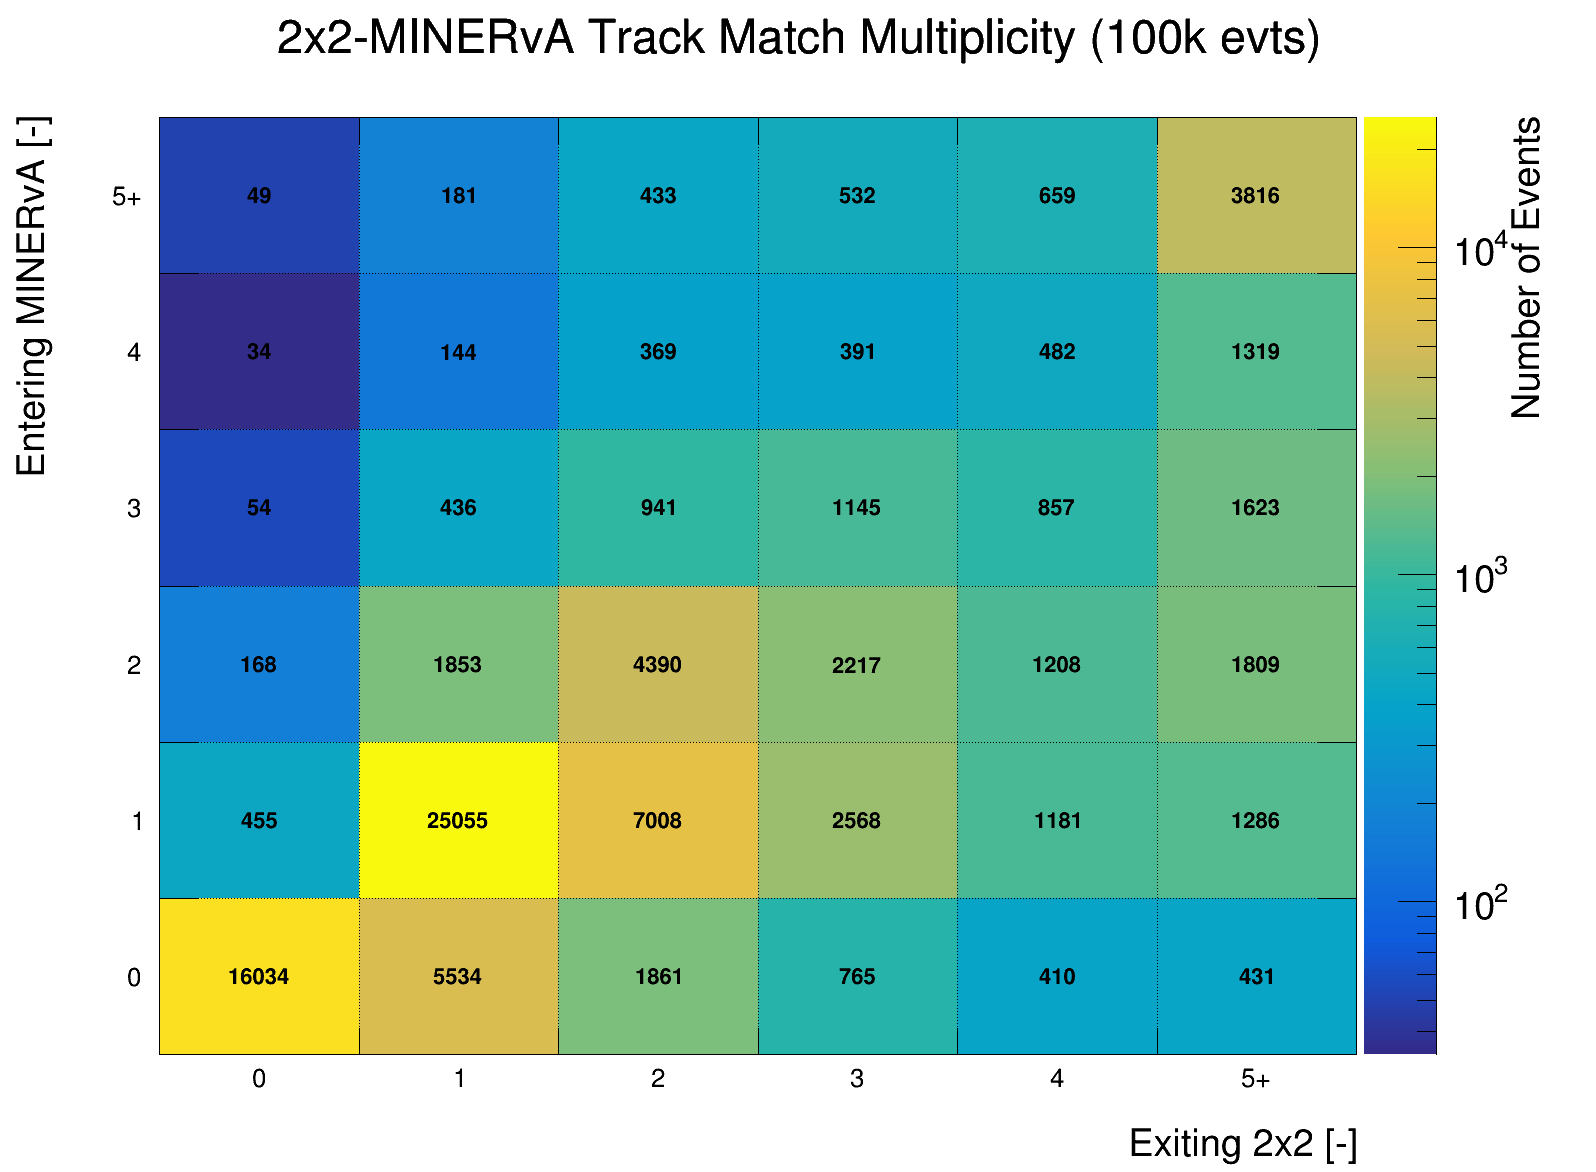
\includegraphics[width=0.6\textwidth]{plots/2x2_minerva_plots/track_mathch_topo.png}
  \caption{Simulated number of true tracks produced by simulated GENIE interactions in the ArgonCube 2x2 active volume, which exit the downstream face of the 2x2 module, relative to the number of tracks which enter the upstream face of the downstream MINERvA component, event by event.}
  \label{fig:track_multiplicity_topo}
\end{figure}
As can be seen from the event display shown in Figure~\ref{fig:2x2+MINERvA_event}, events in which tracks escaping the 2x2 active volume may re-interact in the surrounding LAr bath before entering the MINERvA component included in this simulation, thus making the event more confusing, and difficult to assess reconstruction performance with. Figure~\ref{fig:track_multiplicity_topo} shows the multiplicity of tracks exiting the downstream face of the 2x2 active volume downstream, compared with the number of tracks entering the upstream face of the MINERvA component included in the simulation. The distribution is fairly diagonal, suggesting that although complicated event topologies exist, the events will not be too confused to use for these studies. Note also that this problem could be dramatically reduced by partially instrumenting the dead region between the two detectors.

\subsubsection{Acceptance studies}
\label{sec:minerva-acceptance}
The inclusion of MINERvA in ProtoDUNE-ND will improve the acceptance of particles for various studies. Here, we show how the efficiency for contained events compares for the 2x2+MINERvA setup desribed above, with MINERvA components located downstream of the ArgonCube 2x2 Demonstrator module, and for the 2x2-only case.

\begin{figure}[htb]
  \centering
  \subfloat[2x2-only]    {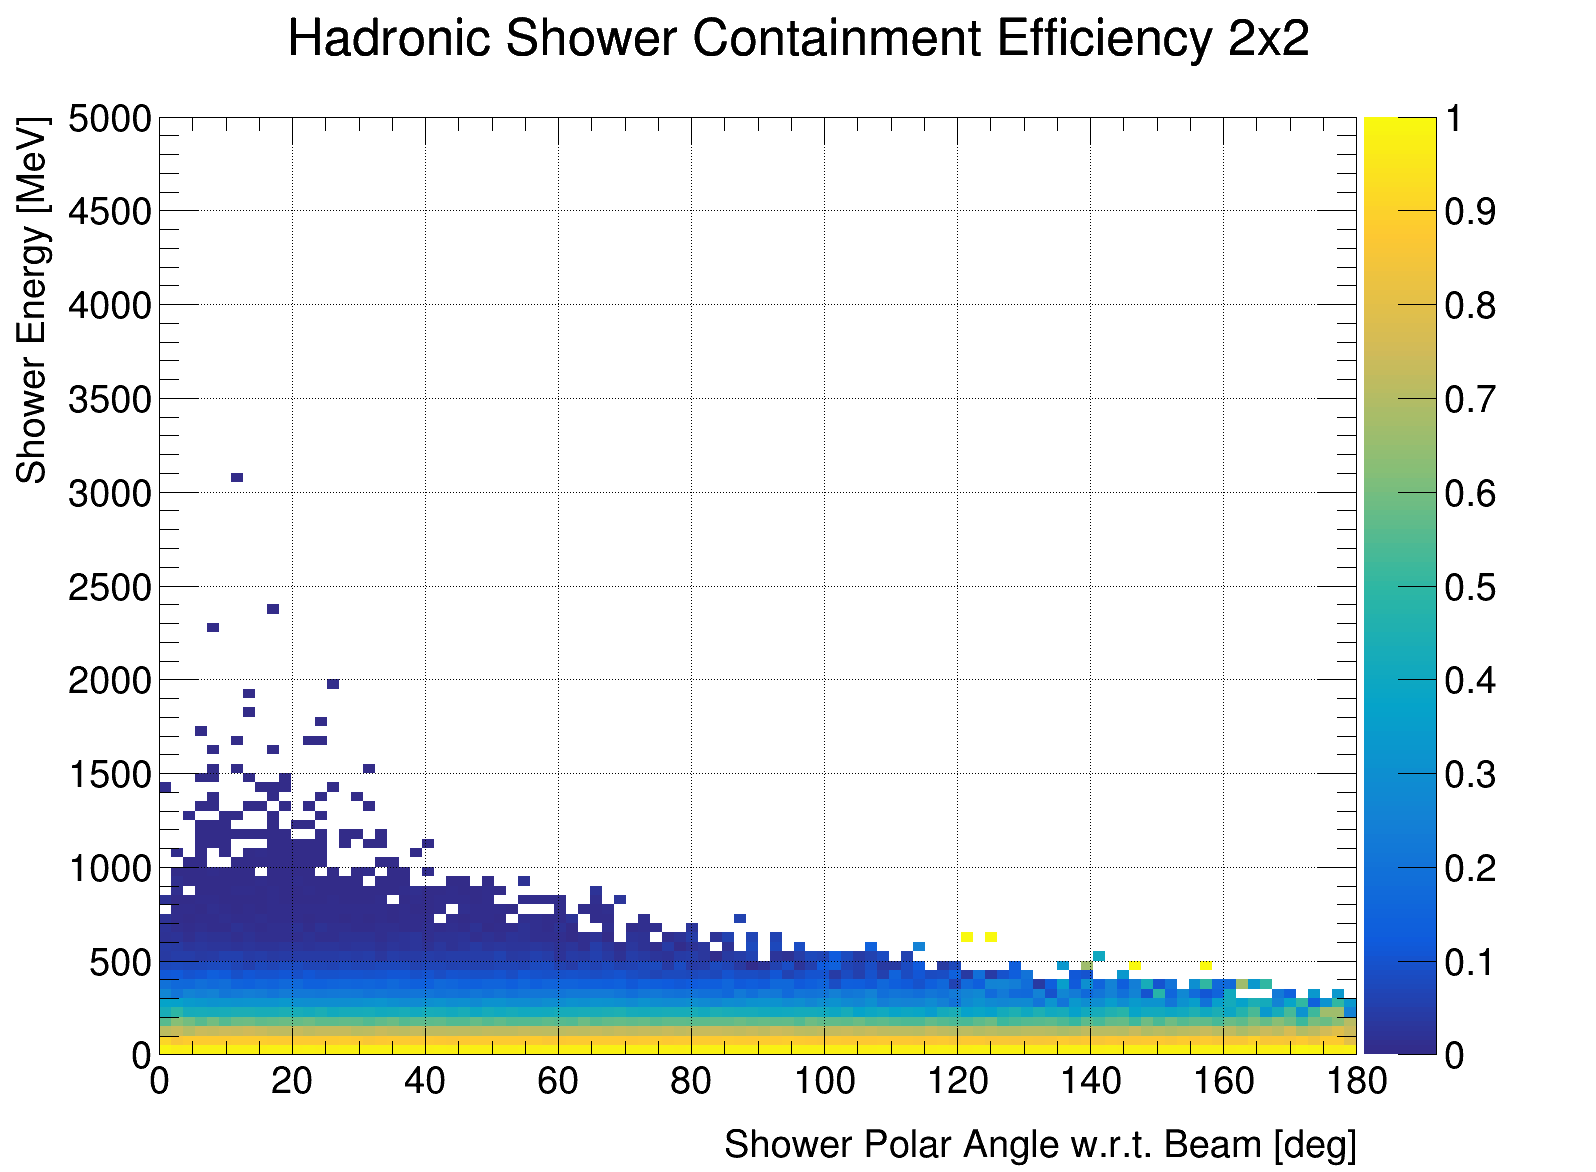
\includegraphics[width=0.45\textwidth]{plots/2x2_minerva_plots/H_cont_eff_2x2.png}}
  \subfloat[2x2+MINERvA] {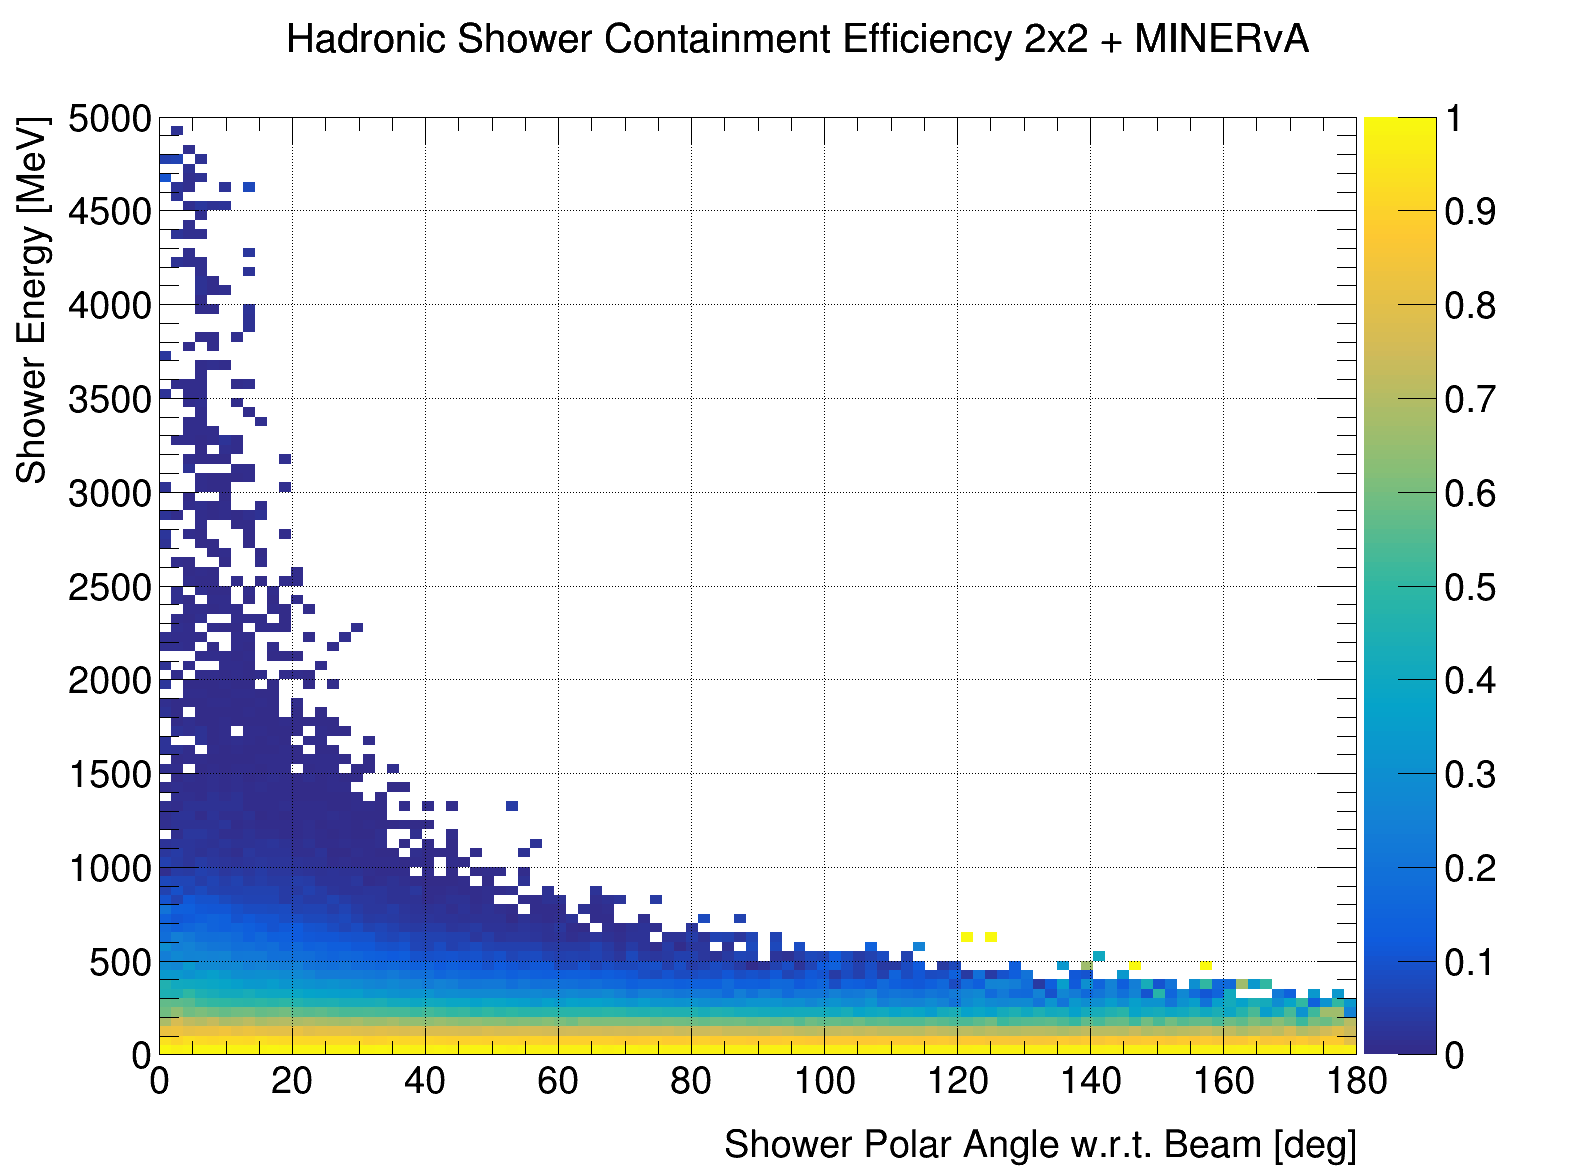
\includegraphics[width=0.45\textwidth]{plots/2x2_minerva_plots/H_cont_eff_2x2_MINERvA.png}}
  \caption{Efficiency for containing hadronic showers, in the 2x2-only, and 2x2+MINERvA, as a function of hadronic shower energy and angle w.r.t the incoming neutrino direction. Containment is defined as $\geq$90\% of the energy being deposited in an active volume of a detector.}
  \label{fig:hadronic_containment}
\end{figure}
In Figure~\ref{fig:hadronic_containment}, the containment of hadron-induced showers is shown as a function of the true energy of the shower, and its angle w.r.t the incoming neutrino beam direction. Showers are defined as being contained when $\geq$90\% of the true energy of the shower is deposited inside the active 2x2 volume, or the MINERvA component if applicable. As expected, including a MINERvA component downstream of the 2x2 module increases the efficiency for angles $\theta \lesssim 30^{\circ}$, which dramatically increases the containment of high energy $E \gtrsim 0.5$ GeV hadronic showers, which tend to be forward-going.

\begin{figure}[htb]
  \centering
  \subfloat[2x2-only]    {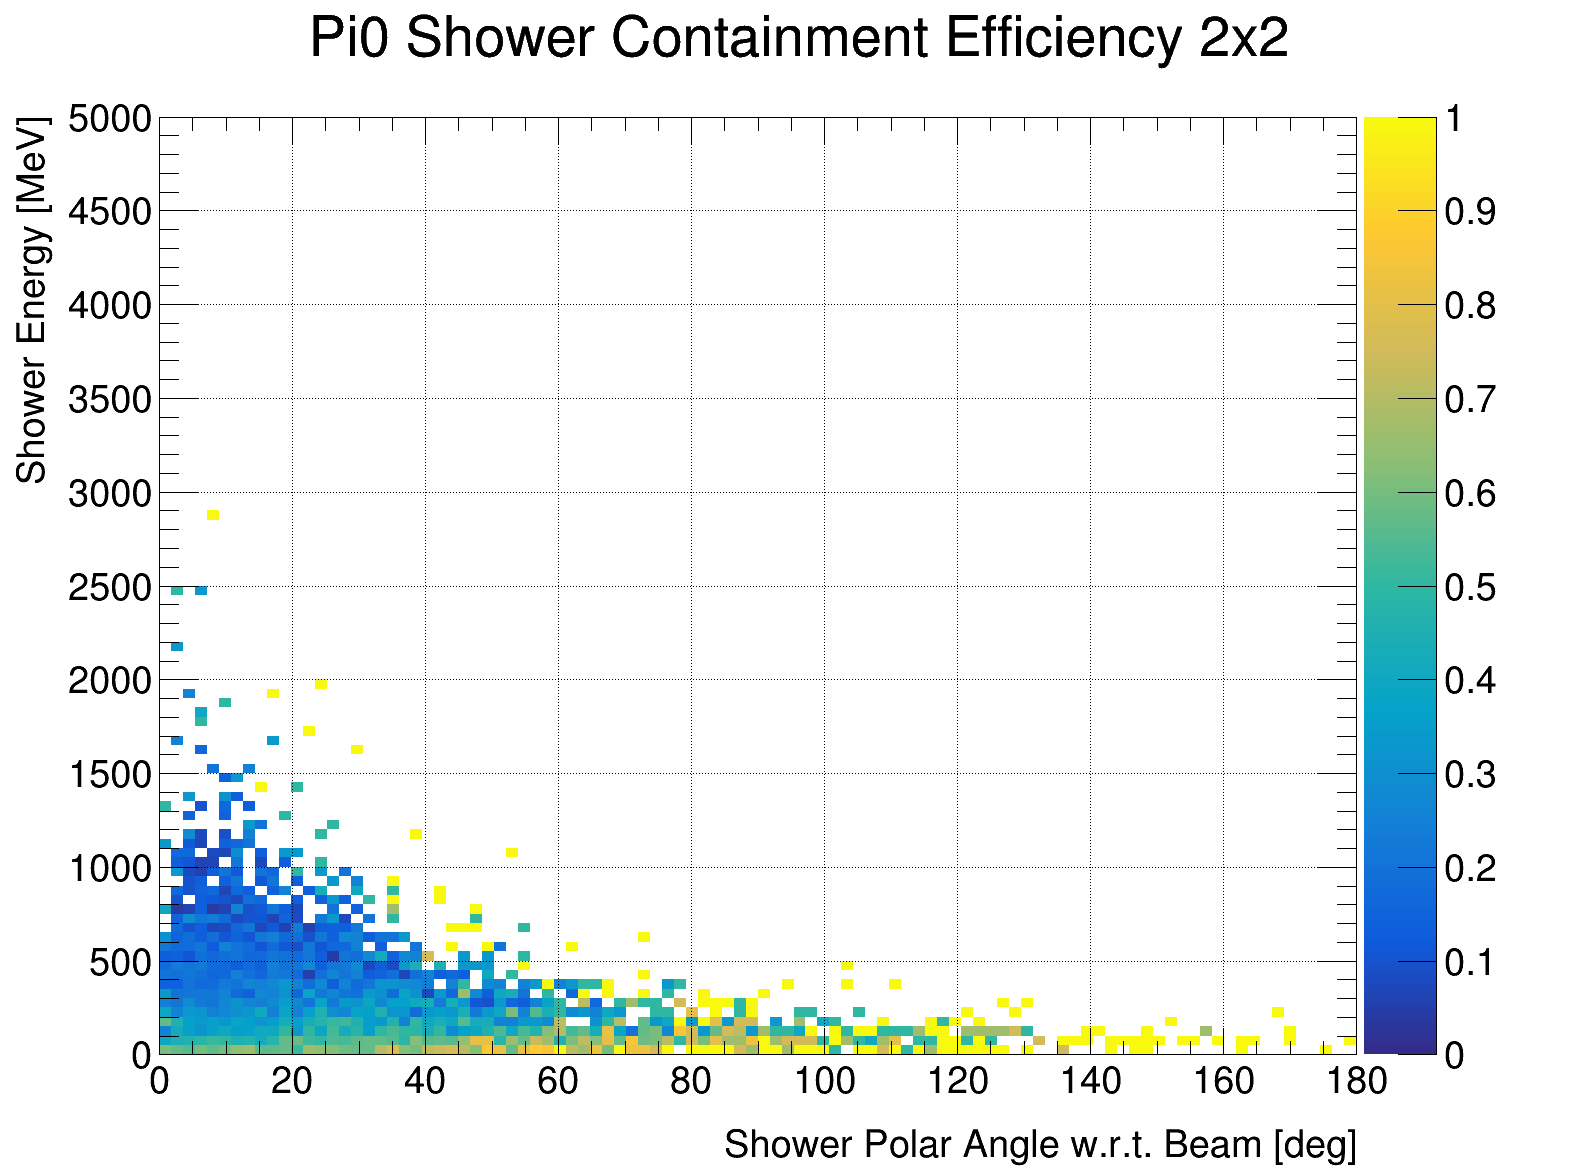
\includegraphics[width=0.45\textwidth]{plots/2x2_minerva_plots/Pi0_cont_eff_2x2.png}}
  \subfloat[2x2+MINERvA] {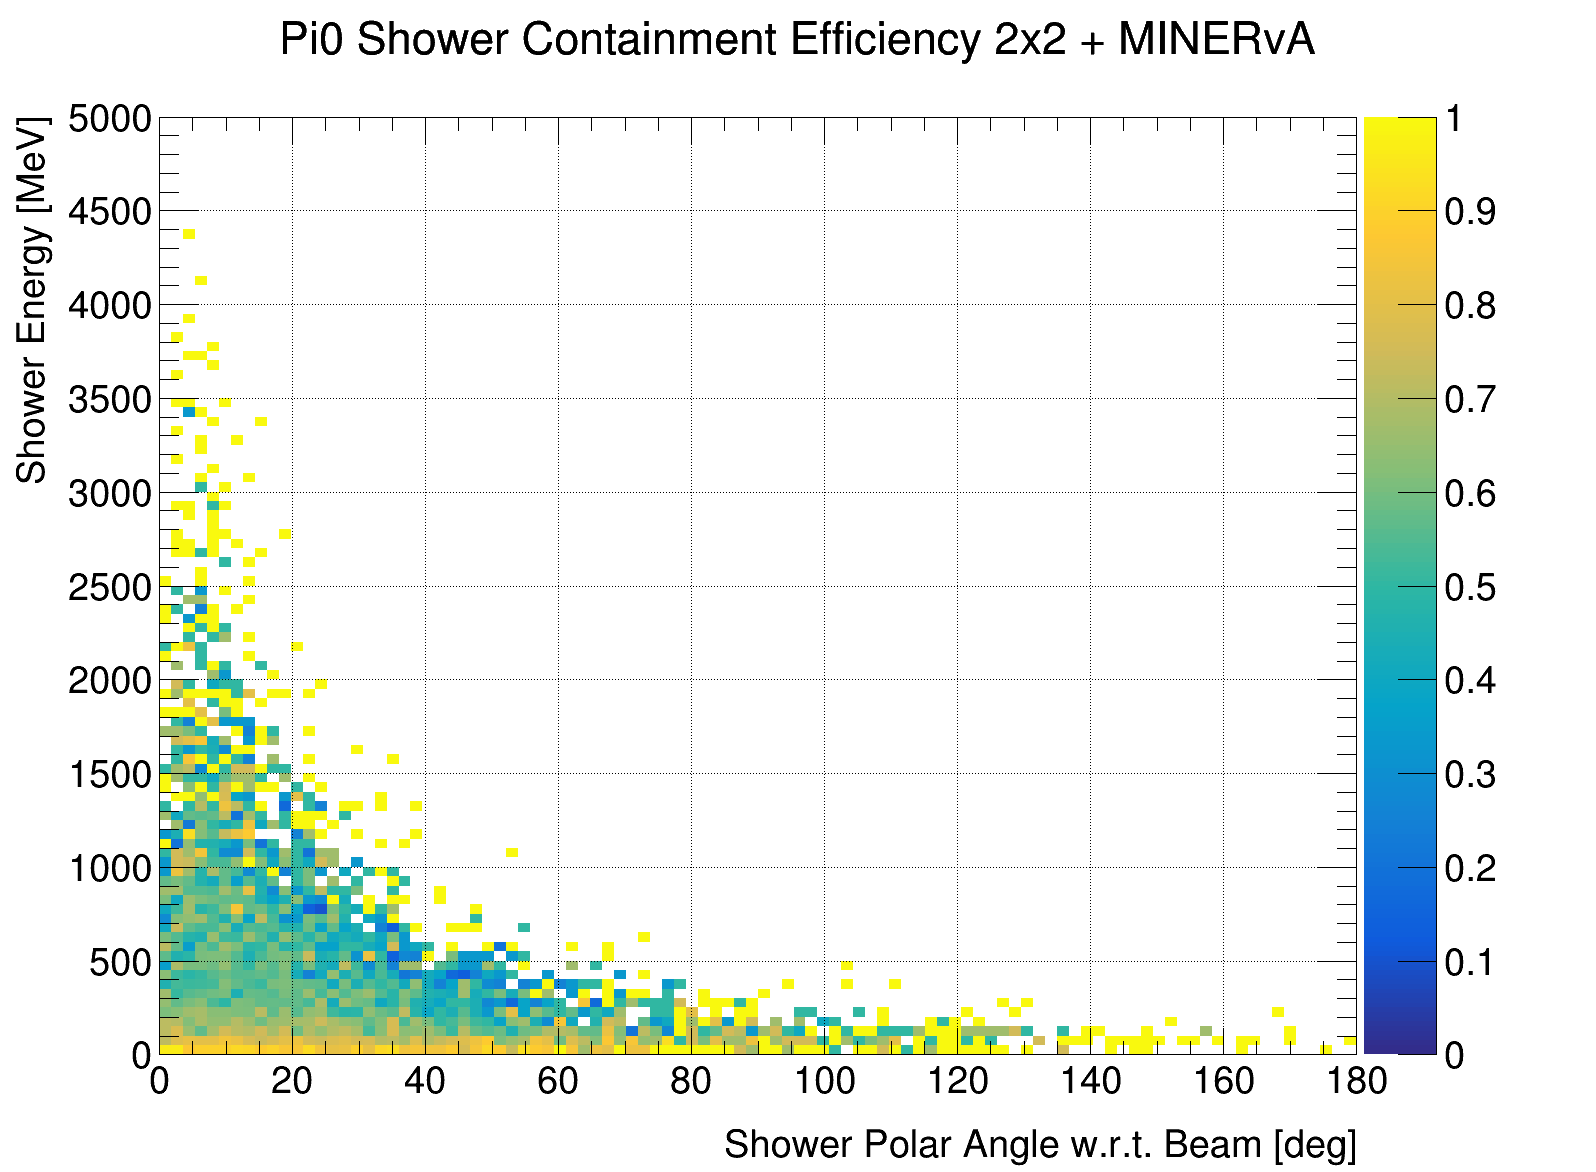
\includegraphics[width=0.45\textwidth]{plots/2x2_minerva_plots/Pi0_cont_eff_2x2_MINERvA.png}}
  \caption{Efficiency for containing both photon-induced showers from $\pi^{0}$ decays, in the 2x2-only, and 2x2+MINERvA, as a function of the $\pi^{0}$ kinetic energy and angle w.r.t the incoming neutrino direction. Containment is defined as $\geq$90\% of the energy being deposited in an active volume of a detector.}
  \label{fig:pi0_containment}
\end{figure}
As discussed previously in this note, as the 2x2 module will not be placed in a test beam prior to installation in the NuMI beam at Fermilab, measurements in which the energy scale of the 2x2 can be calibration will be vital to assess the quality of energy reconstruction in the detector. The containment of both photons from a $\pi^{0}$ decay provides an appropriate in situ measurment of the energy reconstruction capabilities. In Figure~\ref{fig:pi0_containment}, the efficiency to contain 90\% of the energy from both photon-induced showers from a $\pi^{0}$ decay within the active volume of the 2x2, or the MINERvA component if relevant, is shown as a function of the $\pi^{0}$ kinetic energy and angle w.r.t the incoming neutrino beam. There is a significant increase in efficiency for all kinetic energies above a few hundred MeV, particularly for high energy ($E_{\pi^{0}} \gtrsim 1$ GeV) pions, which are produced in the forward direction. Although the dead space between the ArconCube 2x2 active volume and the MINERvA component complicates this picture somewhat, it is clear that including a large portion of MINERvA would give much greater statistics for this benchmark test of the ArgonCube detector performance.

\subsubsection{Neutron tagging studies}

\begin{figure}[htb]
  \centering
  \subfloat[2x2]    {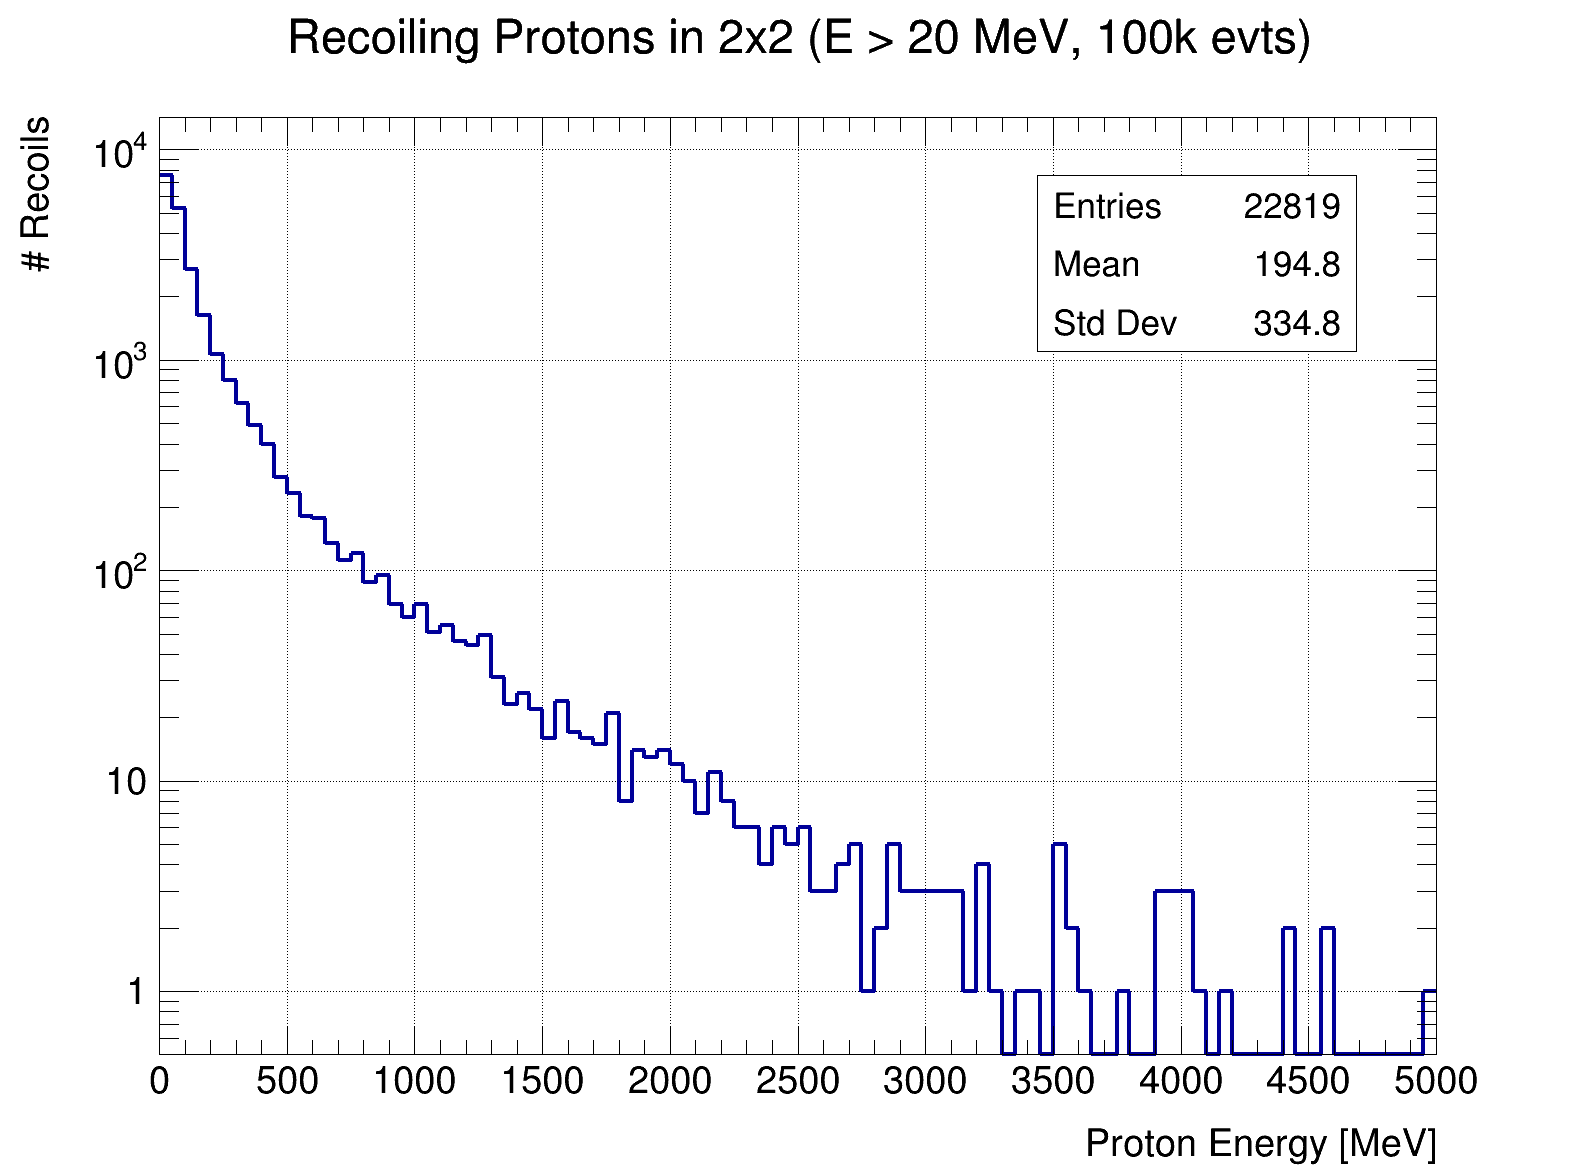
\includegraphics[width=0.45\textwidth]{plots/2x2_minerva_plots/recoils_vs_E_proton_2x2.png}}
  \subfloat[MINERvA] {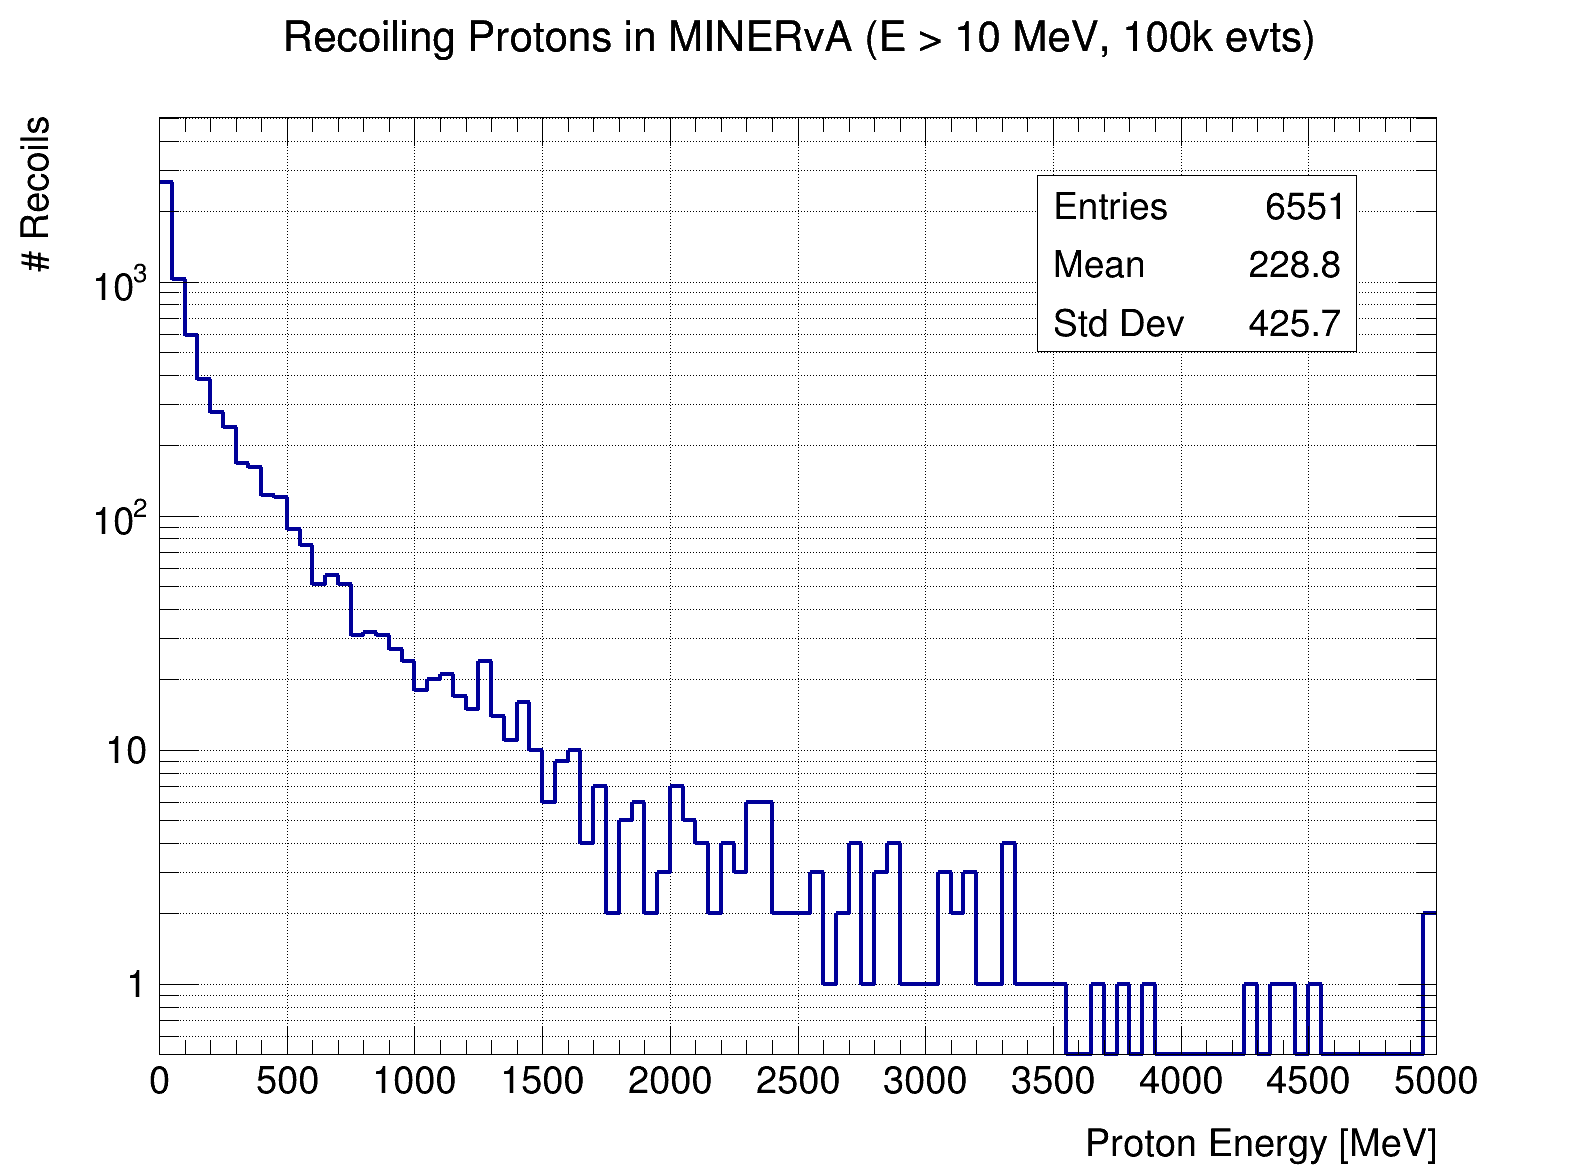
\includegraphics[width=0.45\textwidth]{plots/2x2_minerva_plots/recoils_vs_E_proton_MINERvA.png}}
  \caption{Number of neutron-induced proton recoils as a function of proton energy, which originate from an interaction vertex in the 2x2 active volume, seen in both the 2x2 ative volume, and the downstream MINERvA detector.}
  \label{fig:neutron_tag_minerva}
\end{figure}

As discussed in Section~\ref{sec:2x2_neutron}, one key detector physics goal with ProtoDUNE-ND is to determine whether neutron-induced proton recoils can be identified in a LAr TPC, specifically in ArgonCube. The ability to identify and measure neutrons produced in neutrino interactions is of great interest to DUNE.  At the far detector recoil protons can be identified and easily associated to the neutrino interaction.  However, at the near detector, confusion due to multiple neutrino interactions in the same beam spill poses a unique challenge.  Because neutrons can travel $\mathcal{O}\left(1\right)\,\mathrm{m}$ in LAr without interacting, and proton recoils from fast neutrons typically deposit energy on a single pixel and thus contain no directionality, event association is not possible without matching the charge deposit to an ArCLight optical flash with fast timing resolution.
 
Additionally, it may be possible to measure the neutron energy from time of flight in the DUNE ND using the ECAL with very fast, sub-nanosecond timing resolution. This will require matching muon tracks from either the LAr or HPGAR TPCs to hits in the ECAL to reconstruct the neutrino interaction vertex time with high precision, and also identify and timestamp a subsequent neutron interaction in the scintillator tiles of the ECAL. This would give the DUNE ND unprecedented ability to make measurements of the neutron energy spectrum in neutrino-argon interactions. This technique has not been tested in a high rate environment. Because the neutrons may propagate for $\mathcal{O}\left(10\right)\,\mathrm{ns}$, even a very fast detector may suffer from confusion due to pile-up.

MINERvA can detect neutron-induced proton recoils down to energies of a few MeV, and measure the 3D position of a recoil with a threshold of 20~MeV.  MINERvA has an established neutron reconstruction and a relatively well-understood detector response.  As shown in Fig. 24, it will be possible to reconstruct neutrons originating in the LAr of the ArgonCube 2x2 Demonstrator by their interactions in MINERvA. The ability to match both muons and neutrons originating in LAr to a fast-timing scintillator detector would be a direct test of the feasibility of this technique in DUNE ND. This has profound impact on the design of the ECAL, which would need to be optimized for both EM and neutron reconstruction if this technique is demonstrated to be viable. 
 
 
\FloatBarrier
\subsection{Magnetized low-density tracking detector}
The DUNE ND will employ a downstream tracking detector to measure forward, high-energy muons, and will be sufficiently wide as to contain muons at high angles.  However, for wide-angle muons, tracks will only be contained when the vertex is far from the edges, and will often exit the TPC and not be reconstructed.  This sample could be recovered if the muon momentum can be measured reliably from multiple coulomb scattering (MCS). The far detector will also use MCS for muons which exit the detector.

Such measurements have been carried out in a LAr TPC by MicroBooNE~\cite{Abratenko:2017nki}, although the momentum range is somewhat limited as the only validation sample available is composed of muons which stop in the detector, for which a momentum by range measurement can be made. However, such measurements may be more challenging in a modular TPC such as ArgonCube, where tracks are necessarily broken into segments which are read out separately, and then combined in downstream software.

Although there are only four modules in the ArgonCube 2x2 Demonstrator, each is split into two TPCs, so tracks which exit the downstream face of the 2x2 module may be sampled by up to four independent charge readout planes. With a downstream detector capable of making a precise muon momentum measurement, it would be possible to demonstrate that multiple coulomb scattering will be a viable technique for making momentum measurements in the full ArgonCube deployment in the DUNE ND. Given the hard muon momentum spectrum expected in the NuMI on-axis beam (shown in Figure~\ref{fig:momenta}), it would be hard to make a reliable momentum measurement with a small demonstrator tracker module, or indeed with the MINERvA components proposed in Section~\ref{sec:minerva}, as few would be contained. Such measurements could be made, in the MINOS-ND, which is capable of making momentum measurements for all relevant muon momenta by curvature, or by range.


\section{Cosmic Ray Tagger}

In practice, these panels could be used to better identify a sample of fully contained neutrino events for the studies outlined in Sections~\ref{sec:minerva-acceptance}. Additionally, these cosmic ray tagging modules could then be used to validate space charge build-up and electric field uniformity studies outlined in Section~\ref{sec:efield}, and the cosmic suppression studies described in Section~\ref{sec:cosmic-suppression}, for which an additional scintillator panel would be required.

\subsection{Space charge and electric field uniformity}
\label{sec:efield}
A concern for LAr detectors in a high intensity beam is the build up of space charge --- long-lived argon ions which drift slowly towards the cathode --- and possible affects on the uniformity of the electric field which may accumulate over time. In currently operating and near-future LAr detectors~\cite{Ereditato:2014lra, Antonello:2015lea}, both cosmic tracks and UV lasers are used to calibrate for distortions in the electric field. Both the UV laser track and high energy cosmic muons are expected to leave straight tracks in the detector. If the drift field is not uniform across the detector, ionization electrons produced along the length of this track will not drift at the same speed, or with a constant direction, and will result in a distorted track at the readout plane. By comparing the reconstructed and expected track, a map of the electric field distortion can be built up for calibration purposes.

Assuming that the ArgonCube 2x2 Demonstrator is equipped with scintillator panels to tag cosmic tracks using a timing coincidence between two sides of the detector, and reasonable spatial resolution on those scintillator paddles, electric field distortions could be measured in the 2x2 Demonstrator module. By looking at beam-on, and beam-off data, it would be possible to look at the possible affect of space charge build-up over time due to the high event rate in the NuMI beam. If significant space charge build-up were observed, this would inform the future ArgonCube design for the DUNE ND, as a higher drift field strength would be required.

Additionally, although the electric-field uniformity of the resistive field shell will be checked in a small scale LAr TPC at Bern, a check of the electric-field uniformity and stability over time for full-size ArgonCube modules would be a valuable final validation of the design.

\subsection{Cosmic and Rock Muon suppression}
\label{sec:cosmic-suppression}

The DUNE ND is located underground with a \SI{50}{\metre} overburden, that reduces the cosmic flux by orders of magnitude compared to surface detectors. The cosmic rate in MINERvA (currently in the MINOS ND hall where ProtoDUNE-ND will be sited) is \SI{18}{\hertz}, for $\sim$\SI{6}{\metre\squared}. For the ArgonCube 2x2, in the $\sim$\SI{150}{\micro\second} readout window, assuming $\sim$\SI{2}{\metre\squared}, the rate of cosmics muons is 0.001 per readout window. Reading out around spills only, will result in a coincident cosmic muon once every 20 minutes.
In DUNE ND we expect $\sim$10 rock muons per spill, which will be on average $\sim$\SI{1}{\micro\second} apart in time. They are unlikely to overlap any neutrino activity in 3D, but the fast timing will provide an additional handle.
A key design choice for the DUNE ND is whether or not a muon tagging system is required --- for example, a series of scintillator planes surrounding the LAr TPC, as for SBND and MicroBooNE~\cite{CRT}. The proposed ProtoDUNE-ND test experiment can help inform this design choice, assuming that the ArgonCube 2x2 Demonstrator module is equipped with scintillator paddles.

By using the scintillator paddles to tag cosmic or rock events using a timing coincidence, methods for rejecting them can be validated independently. For example, we expect that the good timing resolution and light localization from ArcLight will allow cosmics out of the beam window to be rejected with a high efficiency. Additionally, if a cosmic muon traverses a pixel plane, or an ArcLight plane, we would expect to see a large charge deposition or a large number of photoelectrons measured, which could be an additional way to reject cosmic muons. Both of these methods can be validated with ProtoDUNE-ND.

\section{Repurposing the MINOS Near Detector}
\label{sec:MINOS}

The MINOS ND~\cite{MINOS_NIM} is a magnetic spectrometer formed of \SI{1}{\kilo\tonne} of steel and plastic scintillator. It is located \SI{2.1}{\metre} downstream of MINERvA in the NuMI beam line, and is now controlled by the MINERvA collaboration, and maintained with Fermilab. A schematic of MINOS ND is shown in Figure~\ref{fig:minos_near_detector}, it consists of 282 planes of \SI{2.54}{\centi\metre} thick steel. Only 152 planes are instrumented with scintillator. Each scintillator plane is made of \SI{1}{\centi\metre} thick  and \SI{4.1}{\centi\metre} wide strips. The most upstream 120 planes form the calorimeter region, where every steel plane is instrumented with scintillator in a central region, and every 5th plane is fully instrumented.  In the downstream spectrometer region, there are no partially-instrumented planes and only every 5th plane is instrumented. The calorimeter alone stops a 5~GeV muon, and the calorimeter combined with the spectrometer stops a 10~GeV muon.

\begin{figure}[htb]
	\centering
	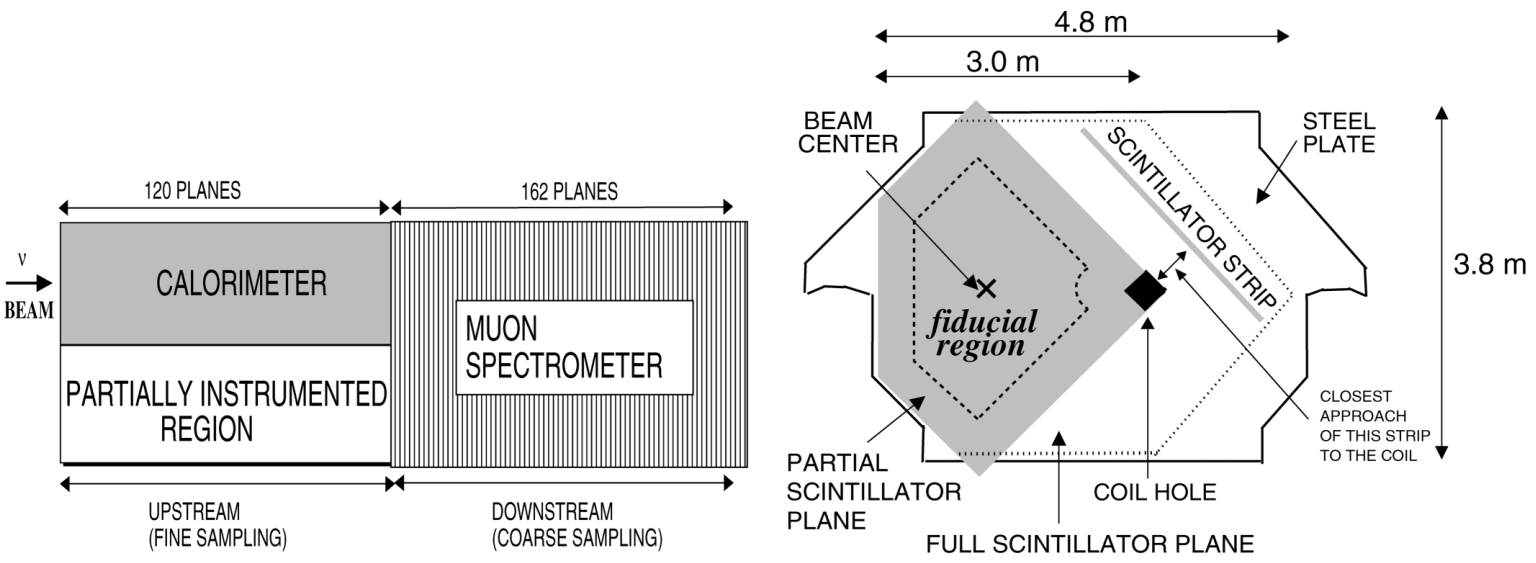
\includegraphics[width=0.9\textwidth]{plots/minos.png}
	\caption{Left: Top view of the MINOS near detector, showing the calorimeter and muon spectrometer (not to scale). Right: transverse view of a near detector plane. The shaded area shows a partially instrumented active scintillator plane and the dashed line within shows the boundary of the fiducial region. The dotted line shows the outline of a fully instrumented scintillator plane. Reproduced from Figure~2 of~\cite{MINOSDetectors}.}
	\label{fig:minos_near_detector}
\end{figure}

As the majority of muons are not contained within the MINERvA volume, and mostly exit downstream, MINERvA currently employ MINOS as a muon spectrometer. Similarly, for ProtoDUNE-ND, the majority of particles will not be contained in the ArgonCube 2x2 volume. Even if MINERvA components are placed downstream of the 2x2 module, the majority of muons will not be contained, making ancilliary physics measurements with ProtoDUNE-ND extremely challenging. Employing MINOS ND as a range finder for ProtoDUNE-ND would allow the muon momentum to be measured, and would allow ProtoDUNE-ND to make much more DUNE-ND-like measurements. If MINOS-ND were to be included downstream, of the MINERvA component, it would also make sense to deploy portions of the MINERvA detector around the ArgonCube cryostat, since the entire MINERvA detector would no longer be needed downstream to maximize momentum sensitivity, making it much easier to tag escaping particles, and to identify through-going cosmics (as alluded to in Section~\ref{sec:cosmic-suppression}), which would make is much easier to calibrate the energy scale in the detector. MINERvA EM scintillator modules could be used to provide vetos for cosmic and rock induced particles entering or exiting the 2x2 cryostat, or to contain side-escaping showers. Ultimately, this would enable a test of the assumption that the DUNE ND does not require a side muon tracker.

Here we discuss such possibilities in brief, and will wait to discover the viability of this project before embarking on more detailed studies. Use of the MINOS ND, in combination with an augmented MINERvA, would allow the reconstruction of the entire properties of an event which occurred in the ArgonCube 2x2 volume. This serves as a proxy for neutrino energy reconstruction, as it would in the full DUNE-ND, and would provide the most thorough calibration of the response of 2x2 possible --- vital, as there are no plans to calibrate the response in a test beam before installation in the MINOS-ND hall at Fermilab.

\subsubsection{Validation of multiple coulomb scattering}

The DUNE ND will employ a downstream tracking detector to measure forward, high-energy muons, and will be sufficiently wide as to contain muons at high angles.  However, for wide-angle muons, tracks will only be contained when the vertex is far from the edges, and will often exit the TPC and not be reconstructed.  This sample could be recovered if the muon momentum can be measured reliably from multiple coulomb scattering (MCS). The far detector will also use MCS for muons which exit the detector.

Such measurements have been carried out in a LAr TPC by MicroBooNE~\cite{Abratenko:2017nki}, although the momentum range is somewhat limited as the only validation sample available is composed of muons which stop in the detector, for which a momentum by range measurement can be made. However, such measurements may be more challenging in a modular TPC such as ArgonCube, where tracks are necessarily broken into segments which are read out separately, and then combined in downstream software.

Although there are only four modules in the ArgonCube 2x2 Demonstrator, each is split into two TPCs, so tracks which exit the downstream face of the 2x2 module may be sampled by up to four independent charge readout planes. With a downstream detector capable of making a precise muon momentum measurement, it would be possible to demonstrate that multiple coulomb scattering will be a viable technique for making momentum measurements in the full ArgonCube deployment in the DUNE ND. Given the hard muon momentum spectrum expected in the NuMI on-axis beam (shown in Figure~\ref{fig:momenta}), it would be hard to make a reliable momentum measurement with a small demonstrator tracker module, or indeed with the MINERvA components proposed in Section~\ref{sec:minerva}, as few would be contained. Such measurements could be made, in the MINOS-ND, which is capable of making momentum measurements for all relevant muon momenta by curvature, or by range.

\subsubsection{Use of MINERvA as a cosmic trigger}
In the discussion in Section~\ref{sec:minerva}, the detector setup maximizes the amount of the MINERvA detector repurposed downstream of the ArgonCube 2x2 module, in order to increase containment in the very forward region, where most particles go. However, if MINOS-ND is also included as part of the ProtoDUNE-ND setup, this imperative is no longer there, and less of MINERvA would be needed downstream. In this case, MINERvA modules could be redeployed to the sides of, and even above, the 2x2 cryostat to act as a cosmic ray or dirt muon tagger, and to tag escaping particles. In practice, these panels could be used to better identify a sample of fully contained neutrino events for the studies outlined in Sections~\ref{sec:minerva-acceptance}. Additionally, these cosmic ray tagging modules could then be used to validate space charge build-up and electric field uniformity studies outlined in Section~\ref{sec:efield}, and the cosmic suppression studies described in Section~\ref{sec:cosmic-suppression}, for which an additional scintillator panel would be required.


\section{MINERvA/MINOS running costs}
\label{sec:costs}

The estimated labor costs for MINERvA infrastructure support, to be repurposed as the ProtoDUNE-ND-Tracker are:
\begin{itemize}
\item 1 person as coordinator and interface with lab computing experts --- 0.5 FTE
\item 1 person as software release and support (Gaudi) --- 0.5 FTE
\item 1 person to monitor keepup --- 0.1-0.25 FTE
\item 2 people for production --- 0.5 FTE (very conservative)
\end{itemize}
Giving a total requirement of 2.1--2.25 FTE, which would have to come from current MINERvA collaborators, not necessarily FNAL employees, who are interested in joining the ProtoDUNE-ND effort. It should be noted that in FY17 MINERvA and MINOS combined used 0.3 FTE from the FNAL Neutrino Division Detector Operations group, and that number would not be expected to rise for the ProtoDUNE-ND-Tracker.

\begin{table}[htbp]
  \centering  
      {\renewcommand{\arraystretch}{1.2}
        \begin{tabular}{cccc}
          \hline\hline
          & & CPU hours & Disk usage (bytes) \\
          \hline
          \multirow{2}{*}{Data} & MINERvA (50\%) & $4.85\times 10^{4}$ & $2.07\times 10^{13}$ \\
          & MINOS & $7.65\times 10^{4}$ & $4\times 10^{12}$ \\
          \hline
          \multirow{2}{*}{MC} & MINERvA (50\%) & $1.8\times 10^{5}$ & $6.3\times 10^{13}$ \\
          & MINOS & $4.5\times 10^{4}$ & $1.3\times 10^{12}$ \\          
          \hline
          \multicolumn{2}{c}{Total} & $3.5\times 10^{5}$ & $8.9\times 10^{13}$ \\
          \hline\hline
      \end{tabular}}  
      \caption{Estimated computing resources required to run MINERvA and the MINOS-ND, assuming that 50\% of MINERvA is retained for the ProtoDUNE-ND-Tracker.}
      \label{tab:minerva-computing}
\end{table}
The expected yearly computing requirement for MINERvA with and without MINOS-ND are shown in Table~\ref{tab:minerva-computing}, assuming that ~50\% of the MINERvA detector is retained and repurposed for ProtoDUNE-ND. Note that it has been assumed that the Monte Carlo production should be ~2$\times$ the data, in keeping with current practice for MINERvA analyses in the NuMI medium energy beam. Note also that the costs in Table~\ref{tab:minerva-computing} do not include those for the ArgonCube 2x2 module. Assuming a cost of \$0.01/CPU hour and \$30/TB, the total cost per year is estimated to be $\sim$\$6000 ($\sim$\$3500 CPU + $\sim$\$2500 disk). Note that in this estimate of computing costs, we have not included the cost of databases and their allocations, or the cost of supporting and maintaining the readout machines.

There are sufficient spare Minder Boards for MINERvA for at least 2 years of operations with the full detector, so there should be plenty of spares given that we would not be using all of the existing MINERvA detector. MINOS front end boards (FEBs) are difficult to replace and prone to failure, however, if the use of MINOS-ND for ProtoDUNE-ND were to be seriously considered, it may be possible to replace the current MINOS FEBs with MINERvA Minder Boards, and still have plenty to spares. This possibility should be seriously considered if the instability of MINOS FEBs are a major issue for this proposal. Of course, the labor cost of such an endeavour would need to be bourne by current MINERvA collaborators wishing to join the DUNE R\&D efforts. 

Finally, the cost of running the detectors themselves has not been considered here. We note that the majority of the power consumption by MINERvA+MINOS-ND is used to run the MINOS-ND magnet. Although the magnet is desirable, it would be possible to use MINOS-ND with the magnet off, at least for some portion of the time, and get momentum estimates by range only.

\section{Conclusions}
\label{sec:conclusions}

In this work, we have outlined the detector physics potential of the ProtoDUNE-ND testbench experiment in the MINOS-ND hall at Fermilab, which is intended to be a ``neutrino engineering'' test. At the heart of ProtoDUNE-ND sits the ArgonCube 2x2 Demonstrator module, which is currently being commissioned, and will be moved to Fermilab by early 2020. The set-up of ProtoDUNE-ND is intended to be flexible, to allow for new modules testing different aspects of the future DUNE-ND design to be installed at different times. This is facilitated by the moveable cryogenic support systems which need to be tested for the DUNE-PRISM baseline design concept, and which will allow the ArgonCube 2x2 to be moved, and the ProtoDUNE-ND arrangement to be reconfigured as a result. The detector physics studies outlined in this document will provide vital inputs to the full-scale DUNE-ND design, and provide a much-needed intermediate scale test, scaling up the small R\&D tests which have already been carried out, and allowing for long-term stability tests to be carried out.

In this document, we have also outlined the detector physics case for incorporating elements of the soon to be decommissioned MINERvA detector into the ProtoDUNE-ND setup, provided all infrastructure and resource availability needs can be met. All DUNE-ND designs considered in Ref.~\cite{dune_ndcsg} include some fast scintillator detector, but no prototype is foreseen at this time for ProtoDUNE-ND. MINERvA components would fill that gap, and provide an essential test of combined reconstruction across different detectors will very different readout technology and times. Additionally, we briefly discussed the possibility to include the MINOS-ND into ProtoDUNE-ND, which is due to be decommissioned along with the MINERA experiment in mid-2019. In combination, using elements of MINERvA and MINOS-ND in ProtoDUNE-ND would allow us to contain all particles in a large fraction of events, and provide a realistic test of the energy recontruction capabilities of the final DUNE-ND. This would be invaluable for DUNE-ND design studies, and would enhance the impact of the ProtoDUNE-ND test.


\printbibliography

%\begin{acknowledgments}
%Thanks for all the \$\$\$
%\end{acknowledgments}


%\bibliography{bibliography.bib}% Produces the bibliography via BibTeX.

%\appendix
%\input{an_appendix}

\end{document}
